\documentclass[11pt,onecolumn]{article}

\usepackage{amsmath}
 \usepackage{titling}
 \usepackage[ruled, vlined]{algorithm2e}
 \usepackage{graphicx}

%\usepackage[T1]{fontenc}
%\usepackage{babel}
\setlength{\droptitle}{-10em}

\title{Reducing the Memory Cost of Training Convolutional Neural Networks by CPU Offloading} % Article title
\author{%
	\textsc{Tristan Hascoet}\thanks{Equal contribution} \thanks{Corresponding author} \\ % Your name
	\normalsize Kobe Univeristy \\ % Your institution
	\normalsize tristan@people.kobe-u.ac.jp % Your email address
	\and % Uncomment if 2 authors are required, duplicate these 4 lines if more
	\textsc{Weihao Zhuang}\footnotemark[1] \\ % Second author's name
	\normalsize Kobe Univeristy \\ % Second author's institution
	\normalsize zhuangweihao1996@gmail.com % Your email address
	\and % Uncomment if 2 authors are required, duplicate these 4 lines if more
	\textsc{Quenti Febvre} \\ % Your name
    \normalsize Sicara \\ % Your institution
    \normalsize quentin.febvre@gmail.com  %Your email address
    \and % Uncomment if 2 authors are required, duplicate these 4 lines if more
    \textsc{Yasuo Ariki} \\ % Second author's name
    \normalsize Kobe Univeristy \\ % Second author's institution
	\normalsize ariki@kobe-u.ac.jp % Your email address
	\and % Uncomment if 2 authors are required, duplicate these 4 lines if more
    \textsc{Tetsuya Takiguchi} \\ % Second author's name
    \normalsize Kobe Univeristy \\ % Second author's institution
	\normalsize takigu@kobe-u.ac.jp % Your email address
}
\date{\vspace{-1ex}}

\begin{document}
	
\maketitle
	
\begin{abstract}

In recent years, Convolutional Neural Networks (CNN) have enabled 
unprecedented progress on a wide range of computer vision tasks. 
However, training large CNNs is a resource intensive task that requires 
specialized Graphical Processing Units (GPU) and highly optimized 
implementations to get optimal performance from the hardware. 
%Given the ubiquity of CNN for practical computer vision applications,
%considerable efforts have been undertaken to optimize their resource consumption.
GPU memory is a major bottleneck of the CNN training procedure,
 limiting  the size of both inputs and model architectures.
%The backpropagation algorithm requires to accumulate the activation 
%values of hidden layers in live GPU memory during the forward pass
%as these activations are needed for the computation of the weights 
%gradient during the backward pass of the backpropagation algorithm.
In this paper, we propose to alleviate this memory bottleneck by 
leveraging an under-utilized resource of modern systems: 
the device to host bandwidth.
%offloading the input activation of hidden layers to the CPU:
Our method, termed CPU offloading, works by transfering hidden activations to the CPU upon
computation, in order to free GPU memory for upstream layer computations during the forward pass. 
These activations are then transfered back to the GPU as needed by the gradient computations of the backward pass.
The key challenge to our method is to efficiently overlap data transfers and computations
in order to minimize  wall time overhead induced by the additional data transfers.
On a typical work station with a Nvidia Titan X GPU and XXX PCIe lanes, 
we show that our method compares favorably to 
gradient checkpointing as we are able reduce the memory consumption of traning a VGG19 model by 35\% with a minimal additional wall time overhead of 21\%. 
Further experiments detail the impact of the different optimization tricks we propose.
Our method is orthogonal to other techniques for memory reduction such as 
quantization and sparsification so that they can easily be combined for further optimizations.

\end{abstract}

\section{Introduction}
% 1. Catchy Intro
Over the last few years, Convolutional Neural Networks (CNN) 
have enabled unprecedented progress on a wide array of computer vision tasks.
One disadvantage of these approaches is their resource consumption: 
Training deep models within a reasonable amount of time requires special
Graphical Processing Units (GPU) with numerous cores and large memory capacity.
Given the practical importance of these models, a lot of research effort has been directed
towards algorithmic and hardware innovations to improve their resource efficiency such as low-precision arithmetic \cite{jacob2018quantization}, network pruning \cite{molchanov2016pruning}, or efficient stochastic optimization algorithms \cite{kingma2014adam}.

% 2. Benefits of low-memory training
In this paper, we focus on a particular aspect of resource efficiency: 
optimizing the GPU memory cost of training CNNs. 
Given the ubiquity of CNN for practical computer vision applications,
optimizing the memory consumption of CNN training has the potential to
impact a wide range of applications. 
Here, we only present a few of the most interesting 
potential impacts of such optimization:

% 2.1 Democratization
\textbf{Low-memory GPUs:} 
Training large CNN requires special GPUs with large memory capacity. 
Typical desktop GPUs memory capacity is too small for training large CNNs.
As a result, getting into deep learning research comes 
with the barrier cost of either buying specialized hardware 
or renting live instances from cloud service providers,
while standard laptop GPUs remain idle untapped resources.
Reducing the memory cost of deep model training allows 
training deep nets on standard graphic cards without 
the need for specialized hardware, effectively removing this barrier cost.

% 2.3
\textbf{Research in optimization:}
Recent works on stochastic optimization algorithms have highlighted the benefits of large batch training \cite{shallue2018measuring,mccandlish2018empirical,you2017large}.
For example, in Imagenet, linear speed-ups in training have been observed 
with increasing batch sizes up to tens of thousands of samples \cite{mccandlish2018empirical}.
Optimizing the memory cost of CNN training may allow further research 
on the optimization trade-offs of large batch training.
Very large batch training on small datasets like MNIST and CIFAR10 is 
computationally inefficient with current stochastic optimization algorithms \cite{mccandlish2018empirical}.
However, for such small datasets, memory optimization would allow to process the full dataset 
in one pass through the networks. 
The ability to process the full dataset in one pass allows to easily train CNNs on the exact gradient of the loss function.
Hence, memory optimization techniques opens the door for research on gradient descent 
optimization of neural networks outside the realm of Stochastic Gradient Descent.

% Paper Overview
% Inherent trade off
There is an inherent trade-off between the memory consumption and computation wall time
of the CNN training procedure:
Existing approaches to optimize the memory consumption of CNN training,
(gradient checkpointing, reversible network architectures),
trade off memory consumption for additional computations by 
recomputing all or a subset of the hidden layers activations during the backward pass.

% Our approach
Instead, our approach reduces the GPU memory consumption without introducing any additional
computation by leveraging an under-utilized resource: host-device communication.
We propose to temporarily offload GPU memory buffers to the CPU during the forward pass 
of the computation, and transfering these memory buffers back into GPU memory as needed by the gradient computations during the backward of the backpropagation algorithm.

% Key challege
They key challenge in our approach is to efficiently overlap the GPU computations
with the data transfers between CPU and GPU in order to minimize the overhead in wall time
introduced by these data transfer.
In this paper, we describe an efficient implementation of this approach that allows us to reduce by
up to 35\% the memory cost of training a VGG network with a minimal wall time overhead of 21\%.
We compare the memory vs. wall time trade off of our approach to gradient checkpointing 
to illustrate the efficiency of our approach.

% Summary
The remainer of this paper is organized as follows: In Section 2, we briefly review the literature for related work.
Section 3 introduces the preliminary notions necessary to understand the root of the GPU memory bottleneck.
Section 4 presents our approach and details the different tricks needed for efficient implementation. 
Finally, Section 5 presents the results of our evaluation.

\section{Related Work}

Research into resource optimization of CNNs covers a wide array of techniques, 
most of which are orthogonal to our work. 
We briefly present some of these works:

% Architecture
On the architectural side, Squeezenet \cite{iandola2016squeezenet} 
was first proposed as an efficient neural architecture 
reducing the number of model parameters while maintaining high classification accuracy.
MobileNet \cite{howard2017mobilenets} uses depth-wise separable 
convolutions to further reduce the computational cost of inference for embedded device applications.

% Pruning & lottery ticket
Network pruning \cite{molchanov2016pruning} is a set of techniques 
developed to decrease the model weight size and computational complexity.
Network pruning works by removing the network weights that contribute the least to the model output.
Pruning deep models has been shown to efficiently reduce the memory 
and computational cost of inference without  significantly hurting model accuracy.
Although pruning methods focus on the optimization of inference, 
the recently proposed lottery ticket hypothesis \cite{frankle2018lottery} 
has shown that specifically pruned networks could  be trained from scratch to high accuracy.
This may be an interesting and complementary line of work to investigate in the future to reduce training memory costs.

% low precision arithmetic.
Low precision arithmetic has been proposed as a mean to reduce 
both memory consumption and computation time of deep learning models.
Mixed precision training \cite{micikevicius2017mixed} combines float16 with float32 operations
to avoid numerical instabilities due to either overflow or underflow.
For inference,  integer quantization \cite{jacob2018quantization,wu2018training} 
has been shown to drastically improve the computation and memory efficiency 
and has been successfully deployed on both edge devices and data centers.
Integrating mixed-precision training to our proposed architecture would allow 
us to further reduce training memory costs. 

% Gradient checkpointing
Most related to our work, gradient checkpointing was introduced as a mean 
to reduce the memory cost of deep neural network training.
Gradient checkpointing, first introduced in \cite{martens2012training}, 
trades off memory for computational complexity by storing only a subset 
of the activations during the forward pass.
During the backward pass, missing activations are recomputed from 
the stored activations as needed by the backpropagation algorithm.
Follow-up work \cite{chen2016training} has since built on the original gradient 
checkpointing algorithm to improve this memory/computation trade-off.  

In contrast, our approach does not induce any additional computation:
Instead of computing a set of missing hidden activations during the backward pass,
we propose to offload the hidden activations to the CPU during the forward pass,
and to transfer these activations back to GPU memory during the backward pass.

Reversible models \cite{gomez2017reversible,jacobsen2018revnet} constrain the CNN architecture to feature invertible transformations.
This allows the activation values of lower layers to be reconstructed from those of higher layers during
the backward pass. 
Reversible networks have been shown to offer a better memory/computation trade-off than 
gradient checkpointing at the cost of constraining the CNN architecture.

Our approach combines revertible operations with CPU offloading:
we use the invertible BN-Leaky ReLu block design proposed in \cite{rota2018place} 
to efficiently deal with normalization and non-linearity layers,
and only offload to CPU the activations of the pooling and convolution layers.

\section{Preliminaries}

Let us consider a model $F$ of $N$ sequential layers trained to minimize an error $e$ 
defined by a loss function $\mathcal{L}$ for an input $x$ and ground-truth label $\bar{y}$:

\begin{subequations}
	\begin{align}
	F &: x \rightarrow y \\
	y &= f_N \circ ... \circ f_2 \circ f_1(x) \\
	e &=  \mathcal{L}(y, \bar{y})
	\end{align}
\end{subequations}

During the forward pass, each layer $f_i$ takes as input the activations $z_{i-1}$ from the previous layer and outputs activation features $z_i=f_i(z_{i-1})$, with $z_0=x$ and $z_N=y$ being the input and output of the network respectively.
During the backward pass, the gradient of the loss with respect to the hidden activations are propagated backward through the layers of the networks using the chain rule as:

\begin{equation}
\frac{\delta \mathcal{L}}{\delta z_{i-1}} = \frac{\delta \mathcal{L}}{\delta z_{i}}  \times \frac{\delta z_{i}}{\delta z_{i-1}}
\end{equation}

Before propagating the loss gradient with respect to its input to the previous layer, 
each parameterized layer computes the gradient of the loss with respect to its parameters. 
In vanilla SGD, for a given learning rate $\eta$, the weight gradients are subsequently used to update the weight values as:

\begin{subequations}
	\begin{align}
	\frac{\delta \mathcal{L}}{\delta \theta_i} & =\frac{\delta \mathcal{L}}{\delta z_{i}}  \times \frac{\delta z_{i}}{\delta \theta_i} \\
	\theta_i & \leftarrow \theta_i - \eta \times \frac{\delta \mathcal{L}}{\delta \theta_i}
	\end{align}
\end{subequations}

For most layers, the computation of either gradients are functions of the layer's input activations $z_{i-1}$:
For example, convolution layers need the values of input activations to compute the weight gradients:

\begin{equation}
\frac{\delta \mathcal{L}}{\delta \theta_i} = z_{i-1} \star \frac{\delta \mathcal{L}}{\delta z_i} 
\end{equation}

while Rectified Linear Unit layers need the input activations values 
to compute the gradients of the loss with respect to its imputs:

\begin{equation}
\frac{\delta \mathcal{L}}{\delta z_{i-1}^j}  = \begin{cases}
\frac{\delta \mathcal{L}}{\delta z_{i-1}^j}, & \text{if}\ z_{i-1}^j \geq 0 \\
0 & \text{if}\ z_{i-1}^j < 0
\end{cases} \\
\end{equation}

Hence, backpropagation implementations in deep learning frameworks
store hidden layers activations in GPU memory 
upon computation during the forward pass. 
Activations accumulate in live memory buffers throughout the full forward pass
until used for gradients computations in the backward pass. 
Once the gradients computed in the backward pass, 
their associated hidden activation buffers can be freed from live memory. 
However, the accumulation of activation values stored within each layer 
along the forward pass creates a major bottleneck in GPU memory.
In the next Section, we detail our approach to alleviate this memory bottleneck.

\section{Propose Method}
\subsection{Framework}

% Describe the ides
The input activations of each layer are kept in GPU memory only to be used for the
computation of the layer weight gradients during the backward pass. 
Hence, the activations of lower layers are kept idle in GPU memory during the
forward and backward computations through higher layers.
We propose to offload these activations to the CPU during this idle time
in order to free up some GPU memory space for the computation of higher layers activations.

% Illustrate with figure
Figure 1 illustrates our approach. 
During the forward pass (top), activations are computed forward through the network layers.
Instead of keeping these activations idle in GPU memory, activation values are transfered to 
the CPU memory immediately after their computation.
In the backward pass (bottom), gradients are backpropagated backward 
through the network layers following equations (3).
Our implementation synchronizes the transfer of the layers input activations back to GPU
right before they are needed for their layer's gradient computation.
Hence the key challenge in our implementation consists in synchronizing the data
transfers with the computations so that only the minimal amount of activation values 
is loaded in GPU memory at any given time, while the least amount of time is spent 
waiting for the data transfer.

\begin{figure}[h!]
\centering
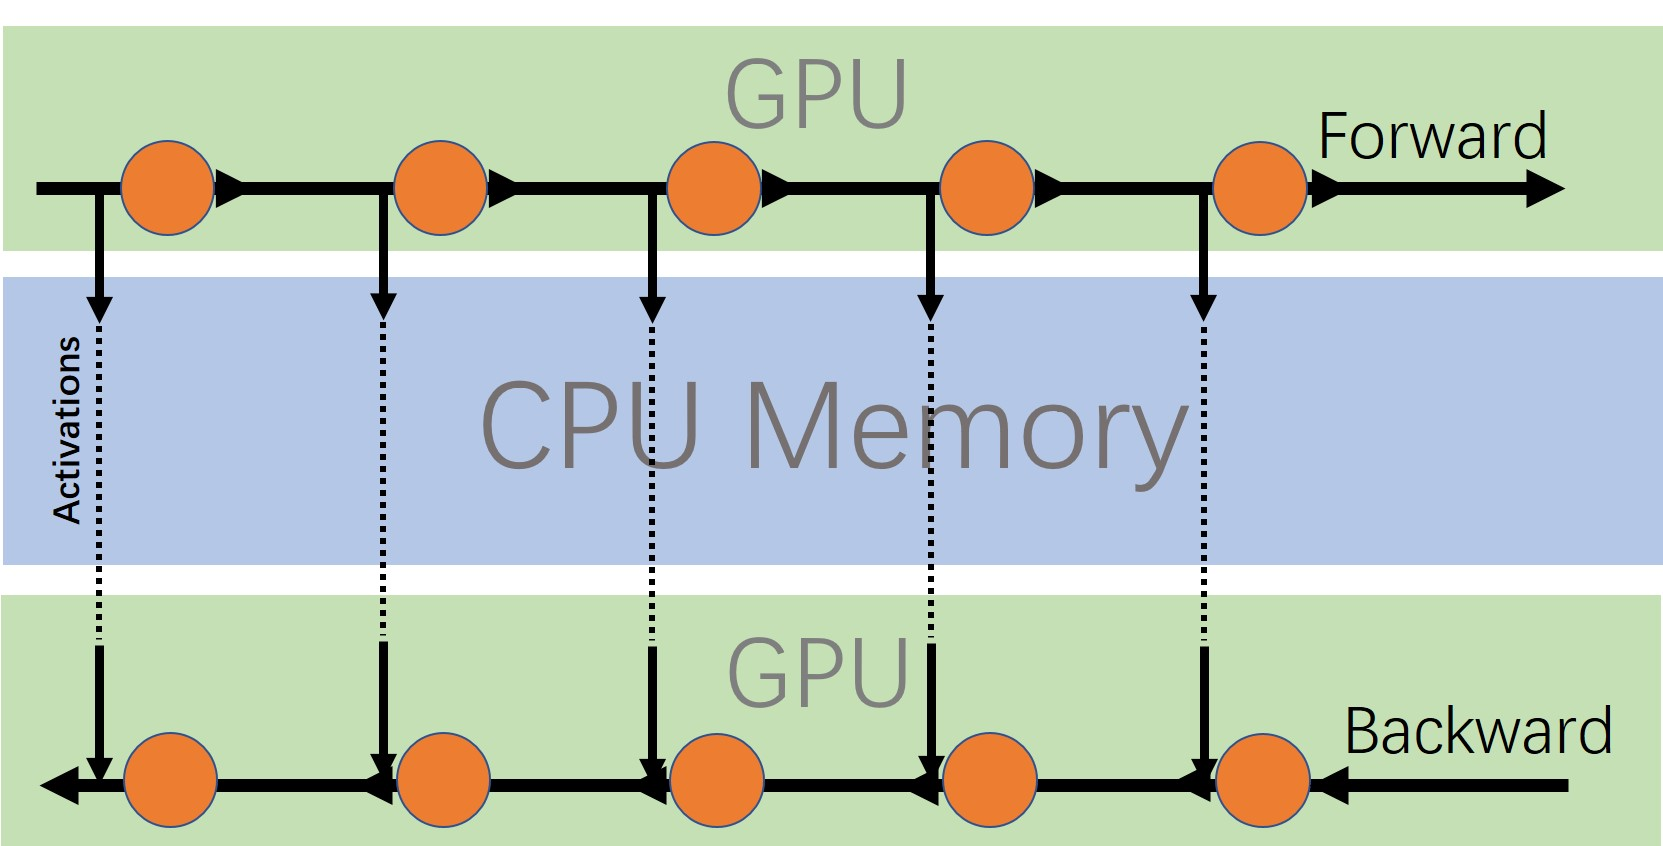
\includegraphics[width=0.8\textwidth]{Figure1.jpg}
\caption{Illustration of CPU Oflloading. 
During the forward pass (top), 
hidden activation buffers are transfered to CPU memory upon computation.
During the backward pass (bottom), hidden activation buffers 
are transfered back to GPU memory just in time to compute the 
weight gradients.}
\end{figure}

% Overview of optimizations
To achieve this goal, we propose a set of optimization tricks organized along two axes:
The first consists in optimizing the data transfer speed between CPU and GPU memory,
using efficient memory accesses and data compression schemes.
The second consists in efficient parallelization to maximally overlap the computations
with the data transfer.
The following subsections details optimizations along these two axes.
% For example, when the forward pass through the first layer completes,  
% our algorithm offloads the input activation of
% first layer to CPU memory and forward its output to the
% second layer. In the backward pass, the input data of each
% layer is transferred back to GPU memory right before
% computation of the weight gradients.

\subsection{Parallelization}

% Idea
Figure 2 illustrates the execution through time of a forward 
and backward pass through a toy network with and without parallelization of the data transfer.
Without parallelization, computation and data transfers are performed sequentially 
so that the total wall time is given by the sum of the computation and data transfer time.
$\mathcal{T}_{total} = \mathcal{T}_{comp} + \mathcal{T}_{data}$
Parallelization aims to overlap the computation and data transfer so that the total wall time is given by
$\mathcal{T}_{total} = \mathcal{T}_{comp} + \mathcal{T}_{idle}$, where $\mathcal{T}_{idle}$ represents synchronization delays in cases where the computation is stopped to await for the required data transfer to complete.

\begin{figure}[h!]
\centering
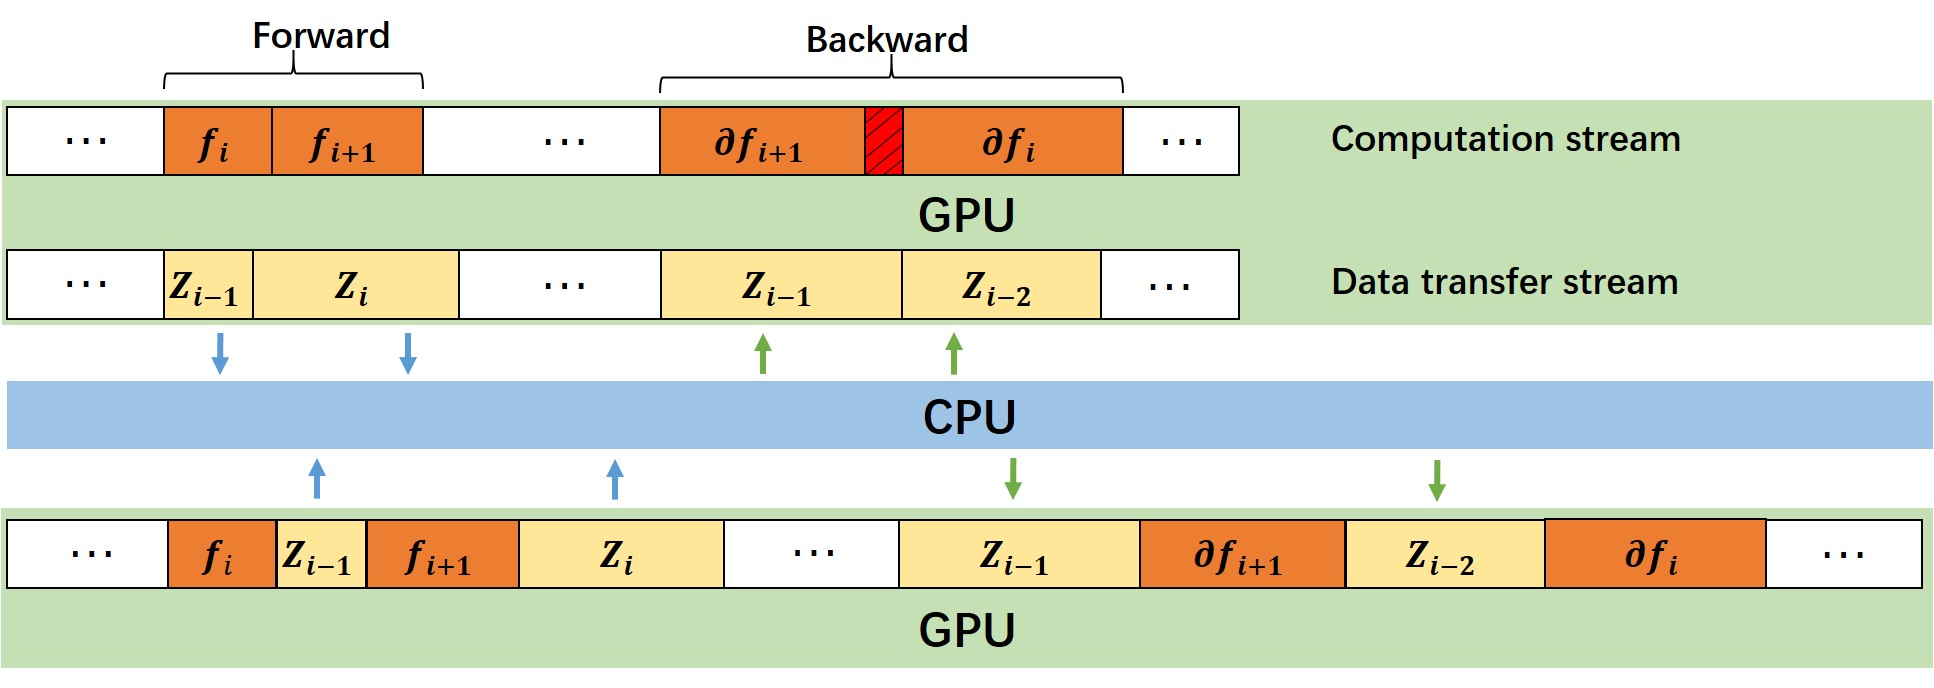
\includegraphics[width=0.8\textwidth]{Figure2.jpg}
\caption{Illustration of the parallel CPU Offloading execution through time.
(top): Computations and data transfer are executed in parallel in their dedicated stream. 
The overhead in wall time $\mathcal{T}_{idle}$ is spent as the computation stream awaits 
for data transfers to complete (illustrated in red). 
(bottom): Without parallelism, computations and data transfers are sequentially executed within the same stream
so that the overhead in wall time corresponds to the total time of data transfers $\mathcal{T}_{data}$}.
\end{figure}


The key challenge in this parallelization scheme consists in efficiently
managaing memory allocation and data transfer so as to
minimize the time $\mathcal{T}_{idle}$ spent awaiting for data transfer.
In this paper, we adopt a simple parallelization strategy:
During the forward pass, activations $z_i$ are transfered to CPU 
upon computation by layer $i$ as $z_i = f_i(z_{i-1})$,
The GPU memory buffer of $z_i$ must then await for both the data transfer to CPU and
the next layer computation $z_{i+1} = f_{i+1}(z_{i})$ to complete before deallocation in order to
avoid unfortunate overwriting by concurrent operations.

\begin{figure*}[h]
\begin{algorithm}[H]
	\KwData{Layer $f_i$, input activation $z_{i-1}$ 
		      \\ \hspace{1.1cm} CPU pinned memory buffer $P_{i-1}$
		      \\ \hspace{1.1cm} CPU thread $T_{data}$
		      \\ \hspace{1.1cm} CUDA events $E_{data}^i$, $E_{comp}^i$
	          \\ \hspace{1.1cm} CUDA Streams $S_{data}$, $S_{comp}$}
\vspace{1mm}
	\KwResult{$z_i$}
\vspace{1mm}
    \textit{Allocate}($z_i$)\;
	$S_{comp} \Leftarrow z_i \leftarrow f_i(z_{i-1})$\;
	$S_{comp} \Leftarrow E_{comp}^i$\;
\vspace{1mm}
	\textbf{In Thread}  $T_{data}$:\\
		\hspace{1.1cm} 	$S_{data} \Leftarrow P_{i-1} \leftarrow z_{i-1}$\;
		\hspace{1.1cm}  $S_{data} \Leftarrow E_{data}^i$\;
		\hspace{1.1cm}  \textit{Wait}($E_{data}^i$, $E_{comp}^i$)\;
		\hspace{1.1cm}  \textit{Free}($z_{i-1}$)\;
	\caption{Forward procedure through layer $i$ with parallel CPU offloading. }
\end{algorithm}
\small{Algorithm 1: Double arrows indicate the asynchronous execution of a CUDA directive within a stream.
Data transfers are executed within dedicated CUDA stream and CPU thread to
synchronize the memory deallocation without blocking the execution of upward layers}
\end{figure*}


One important exception to this rule concerns skip connections, as illustrated in Figure 3.
Skip connections induce a delay in the GPU buffer dealocation as the input of residual blocks must
be kept in memory until the end of the residual block computation to be added to the output.
In ResNet architectures, this delay is short enough to have little impact on the memory/wall time trade off.
However, this means that our method is poorly suited to densely connected 
networks such as DenseNet \cite{huang2017densely} or UNet \cite{ronneberger2015u}, which features very long skip connections.

%() In the experiment section, we will show that this delay slightly degrades the memory consumption 
%of CPU offloading for residual networks compared to sequential architectures like VGG.
%Synchronization of the computation and data transfers during the backward pass is slightly more complicated:

During the backward pass, the input activation $z_{i-1}$ 
of layer $i$ must be transferred back into GPU memory
for the backward gradient computations to proceed.
Hence, we overlap the transfer of $z_{i-1}$ to GPU 
with the backward computations of the upper layer $i+1$ to avoid GPU idle time.
As formalized in Algorithm 2, we thus synchronize the data transfer of $z_{i-1}$ 
with the beginning of the backpropagation through $f_{i+1}$.

\begin{algorithm}[h]
	\KwData{Layer $f_i$, output gradients $\frac{\delta \mathcal{L}}{\delta z_{i}}$
		\\ \hspace{1.1cm} CPU pinned memory buffer $P_{i-1}$
		\\ \hspace{1.1cm} CPU thread $T_{comp}$
		\\ \hspace{1.1cm} CUDA events $E_{data}^i$, $E_{data}^{i+1}$}, $E_{comp}^{i}$
     	\\ \hspace{1.1cm} CUDA Streams $S_{data}$, $S_{comp}$%\\
	\vspace{1mm} \\
	\KwResult{$\frac{\delta \mathcal{L}}{\delta z_{i-1}}$, $\frac{\delta \mathcal{L}}{\delta \theta_i}$}
	\vspace{1mm}
	%\textit{Free}($z_{i}$)\;
	\textit{Allocate}($z_{i-1}$)\;
	\vspace{1mm}
	$S_{data} \Leftarrow z_{i-1} \leftarrow P_{i-1}$\;
	$S_{data} \Leftarrow E_{data}^i$\;
	\vspace{1mm}
	\textit{Wait}($E_{data}^{i+1}$)\;
	\textit{Allocate}($\frac{\delta \mathcal{L}}{\delta z_{i-1}}$, $\frac{\delta \mathcal{L}}{\delta \theta_i}$)\;
	\vspace{1mm}
	$S_{comp} \Leftarrow \frac{\delta \mathcal{L}}{\delta z_{i-1}} \leftarrow \frac{\delta \mathcal{L}}{\delta z_{i}}  \times \frac{\delta z_{i}}{\delta z_{i-1}}$\;
	$S_{comp} \Leftarrow \frac{\delta \mathcal{L}}{\delta \theta_i} \leftarrow \frac{\delta \mathcal{L}}{\delta z_{i}}  \times \frac{\delta z_{i}}{\delta \theta_i}$\;
	\caption{Backward procedure through layer $i$ with parallel CPU offloading.}
\end{algorithm}

We use threading and locks to handle the parallelism and synchronization on the CPU side,
and CUDA streams to handle the parallelization on the GPU end. 
CUDA events provides synchronization primitives to precisdely track 
the completion of kernel executions.
Algorithm 1 and 2 provide pseudo-code for the forward and backward pass respectively.

\begin{figure}[h]
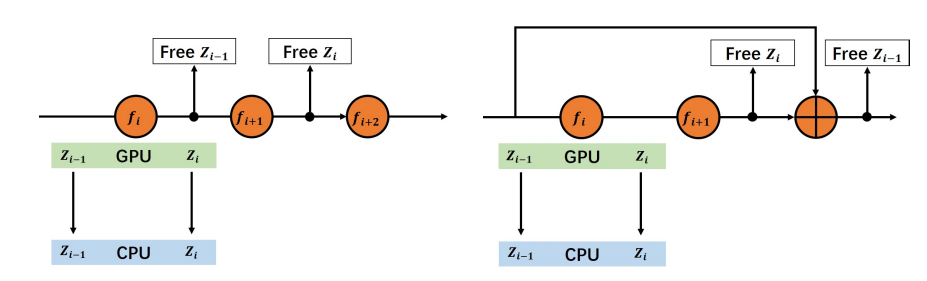
\includegraphics[width=\textwidth]{Figure3.png}
\caption{Illustration of the delay in memory deallocation induced by residual connections.
(left) without residual connection, the input $z_{i-1}$ of layer $f_i$ can be freed from GPU memory 
as $f_i$ computation terminates. 
(right) Residual connections induce a delay in memory deallocation
as $z_{i-1}$ must be kept in GPU memory to be added to the ouput of the residual block. 
}
\end{figure}

% Discussion on compute time vs. transfer time.
With the above parallelization scheme, the overhead $\mathcal{T}_{idle}$ in wall time 
is given by the sum of the difference in the computation and data transfer time at each layer.
If data transfer is faster than the computation in each layer, 
CPU offloading will reduce memory consumption without any overhead in wall time.
Hence, CPU offloading is best suited for computation intensive operations like convolution.
In contrast, batch normalization layers come with negligible computational cost,
but significant data transfer time so that offloading the input activations of 
such layer comes with a significant overhead.
Instead of offloading these layers, we reconstruct their input activations 
from their output using their inverse operation, as proposed in \cite{rota2018place},
and only offload the input activations of the convolution and pooling layers to CPU. 

 \subsection{Data Transfer Optimization}
% Intro
The time needed to transfer data between devices is given by the product of the
transfer speed bandwidth $\mathcal{B}$, in bytes per second, by the volume 
$\mathcal{V}$ of the data buffer in bytes:

\begin{equation}
\mathcal{T}_{data} = \frac{\mathcal{V}}{\mathcal{B}}
\end{equation}

Hence, minimizing data transfer time can be achieved by either
maximizing the transfer speed $\mathcal{B}$ or minimizing
the activation volume $\mathcal{V}$ through data compression.
In this paper, we focus on maximizing data transfer speed using pinned
CPU memory buffers.

% Pinned Memory
CPU memory can be accessed through either pageable memory 
or pinned memory address spaces.
Pinned memory allows for Direct Memory Access (DMA), 
which can significantly speedup data transfer between CPU and GPU devices through PCIe lanes.
However, allocating pinned memory buffers is a time consuming operation, as illustrated in Table 1.
Hence, naively allocating pinned memory buffers within each forward pass would
slow down training due to the overhead of pinned memory allocation.
Instead, we propose to allocate the pinned memory buffers beforehand, 
during the initialization of the CNN.
Our implementation scans the network architecture upon instantiation
and allocates dedicated pinned memory buffers for each 
target layer activations (convolutions and max-pooling). 
During the forward pass, we transfer the GPU data directly into the pre-allocated pinned memory buffer,
and, during the backward pass, we transfer the activations back to GPU from these pinned buffers.
Table 1 quantifies the gains in transfer speed brought by the use of pinned memory buffers, and in Section5, we evaluate the impact of using pinned memory buffers on the overall efficiency of our method.

\begin{table*}[t]
\begin{center}
\begin{tabular}{ c c }	
\hline
Operation     & Speed (GB/s)  \\
\hline
Pinned Memory Allocation     		&  $1.95$        \\
GPU $\rightarrow$ CPU (Pageable)	&  $1.75$        \\
GPU $\rightarrow$ CPU (Pinned)	        &  $6.5$          \\
CPU $\rightarrow$ GPU (Pageable)	&  $4.1$          \\
CPU $\rightarrow$ GPU (Pinned)	        &  $6.1$          \\
\hline
\end{tabular}
\caption{Measurement of data transfer and pinned memory allocation speed on our workstations.
Pinned memory buffers bring a substantial speed up in both directions of the data transfer.}
\end{center}
\end{table*}

% Compression
Another way to reduce the time of data transfer between CPU and GPU is to minize 
$\mathcal{V}$ by compressing the hidden layer activations 
before transferring them between devices.
Compression can be achieved by diverse means including sparsification, 
quantization or low rank factorization techniques.
Low-rank factorization would induce non-negligible additional computational costs, 
which would slow down the computation.
Either sparsifying or quantizing the layers activations are interesting solutions.
However, compression would incur minor losses of precision in the activation values,
which might affect the training dynamics.
Although previous works suggest that such minor losses in precision does not negatively impact training,
investigation of compression techniques would require a detailed analysis 
of the impact of compression on accuracy, which is out of the scope of this paper.
Hence we leave this question open for future work as an interesting direction for further optimization.

\section{Experiments}

% Describe system setup.
We conduct our experiments on a workstation with an NVIDIA Titan X GPU connected 
to the host through XXX PCIe lanes, which represents a peak bandwidth of XXXB/s.
We believe this set-up to be representative of a typical workstation for individual practioners, 
if not slightly unfavorable, as our device to host bandwidth is rather limited.
Unless specified otherwise, we condut our experiments on a batch of 32 RGB images 
with a resolution of 128 by 128 pixels.
For each experiment, we are interested in the total memory usage and Wall time of
the computation for a full training iteration including the forward and backward pass through the network.
It is important to note that our method does not modify the actual computations performed
by the network so that the training dynamics and accuracy are unaffected by CPU Offloading.
Hence, we focus on reporting the memory vs. wall time trade-off,
 as the accuracy reached by the model is strictly unaffected.

\subsection{Memory vs. Wall Time Trade-Off}

Our implementation allows to control for the memory foot-print vs. computation wall time trade-off by 
either using more agressive parallelization schemes,
or by offloading different subsets of hidden layers input activations.
In this section, we use the parallelization scheme described in Section 4.2
and explore the memory vs. time trade-off by off-loading different subsets of the model's layers.

Figure 4 compares the memory/Wall time trade-off of CPU off-loading
to the trade-off provided by gradient checkpointing,
as implemented in the Pytorch \cite{paszke2017automatic} library on the VGG19 architecture.
In gradient checkpointing, this trade-off is defined by the
number of checkpointed layers through the full architecture.

\begin{figure}[h!]
\centering
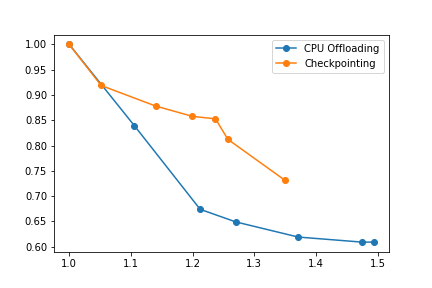
\includegraphics[width=0.5\textwidth]{Figure4.png}
\caption{Comparison of the memory vs. Wall time trade-off achieved by CPU Offloading and sequential gradient checkpointing.}
\end{figure}

% Figure of memory/time trade-off comparison.
Figure 4 shows the pareto frontier for an extensive search
in both checkpointing and CPU offloading layer subset.
CPU offloading leads to a better trade-off between memory consumption and wall time.
This observed performance is due to the fact that the data transfer between host and device
can be efficiently parallelized with the computation, hence incurring a minor overhead,
while gradient checkpointing can not parallelize the gradient computations and activation reconstructions.
Hence, the additional cost of sequentially reconstructing the hidden activations 
during the backward pass induces a higher overhead.

\subsection{Ablation study}

Table 2 illustrates the speed up brought by both parallelization and pinned memory buffers.
We record the timings of a training iteration needed to achieve maximal 
memory reduction on the VGG19 architecture for an input batch of 32 images with 218 by 128 pixel resolution.
We start by recording the time for a baseline CPU offloading approach without parallelization 
nor data transfer optimization.
We then successively integrate the pinned memory buffers and parallelization to this baseline 
and observe the improvement.

\begin{table*}[h]
\begin{center}
\begin{tabular}{ c c c}	
\hline
Operation                   & Time (ms)  & Rel. Improvement\\
\hline
Baseline                    &  $560$    & $0\%$      \\
Pinned Memory               &  $355$    & $-xxx\%$ \\
Parallelization             &  $236$    & $-xxx\%$ \\
\hline
\end{tabular}
\caption{Speed-ups achieved by the pinned memory buffers and parallelization techniques}
\end{center}
\end{table*}

Both parallelization and pinned memory buffers bring substantial improvements 
in speed and have proven critical for performance.
Compression of the hidden states to either sparse representations or lower precision
encodings may bring similar speed-up and would be very interesting to investigate in future work. 	
We expect that simply converting the hidden activations to FP16 before sending them
to the host device should further reduce the data transfer by half.

\subsection{Architecture comparison}

In this section, we compare the memory gains and time overhead 
achieved through CPU offloading on different popular architectures.

\begin{table*}[h]
\begin{center}
\begin{tabular}{ c c c}	
\hline
Architecture            & Wall Time Overhead & Memory Reduction    \\
\hline
VGG16                   &  $19.5\%$            & $32.5\%$          \\
VGG19                   &  $21.0\%$            & $36.9\%$          \\
Resnet18       	        &  $17.6\%$            & $54.4\%$          \\
Resnet50                &  $15.3\%$            & $56.8\%$          \\
MobileNet               &  $63.2\%$            & $67.8\%$          \\
\hline
\end{tabular}
\caption{Memory vs.Time trade-off achieved by different architectures.
The Wall Time Overhead column shows the additional time needed to achieve the given memory reduction (the lower the better).
Memory Reduction represents the reduction of peak memory usage achieved with CPU offloading (the higher the better).}
\end{center}
\end{table*}

Both ResNet architectures and MobileNet \cite{howard2017mobilenets} feature batch normalization layers, 
for which we used the invertible operation of \cite{rota2018place}. 
Invertible batch normalization layers further reduce the memory consumption 
with little time overhead, which explains the slightly better trade-off of ResNet architectures.
On the other hand, the MobileNet architecture uses depth-wise convolutions instead of the 
reguar convolution layers used in both VGG and ResNet architectures.
Depth-wise convolutions have lower arithmetic intensity \cite{wu2018shift} than convolution layers,
i.e.; for input activations of similar size, they perform less, hence faster, operations. 
As computations are performed faster while the data transfer time remains constant,
CPU offloading of depth-wise convolutions incur a more important overhead.
This result highlights the fact that CPU offloading works best for computationally
intensive layers.

\subsection{Discussion}

The memory/time trade-off achievable by CPU offloading is a function of the ratio 
between computation and data tranfer speed. 
This ratio varies with the specific hardware
being run on, the algorithm used for the convolutions, 
as well the efficiency of their implementation.

On the software side, the experiments presented in this paper were run 
with state-of-the art cudnn implementations of the winograd convolution 
algorithm through the PyTorch framework \cite{paszke2017automatic}.
On the hardware side, we ran experiments on a single 
Nvidia Titan X GPU connected to the host via a 6GB/s bandwitdth connection, 
which we believe to be representative of a typical deep learning student/researcher's workstation.

The exact trade-offs achieved will differ depending on the specific hardware and software used in 
different systems, as well as the parallelization strategy used for CPU offloading. 
However, the fact that data transfers between CPU and GPU can be efficiently parallelized with the GPU computations
means that memory gains can be achieved with minimal time overhead 
on any sytem given an appropriate parallelization strategy.  

Searching for an optimal parallelization strategy given a fixed computational graph and hardware system
is a very interesting problem left open to investigate. 
In this paper, we provide a proof of concept by showing that 
even a rather naive parallelization strategies with minimum optimization
leads to a memory/time trade-off competitive relative to 
the well established method of gradient checkpointing.

\section{Conclusion}

Convolutional Neural Networks have become the backbone of computer vision systems.
Despite their great success, one major drawback of these models is their intense resource consumption:
Training CNNs needs highly optimized implementations leveraging all possible hardware resources.
In this paper, we proposed to leverage GPU-CPU communication, 
an under-utilized resource in typical CNN training pipelines,
to alleviate the GPU bottleneck in training CNNs. 
Our experiment on a standard single-GPU work station shows a more
effective memory/wall time trade-off than gradient checkpointing.
Our approach is orthogonal to other resource optimization approaches 
such as pruning, quantization so these approaches can easily be combined in future work.

\bibliographystyle{unsrt}
\bibliography{article}

\end{document}
	
